\documentclass[12pt, a4paper]{article}

% ── Packages ──────────────────────────────────────────────────────────────────
\usepackage[utf8]{inputenc}
\usepackage[T1]{fontenc}
\usepackage[english]{babel}
\usepackage{geometry}
\usepackage{amsmath, amssymb}
\usepackage{graphicx}
\usepackage{float}
\usepackage{booktabs}
\usepackage{hyperref}
\usepackage{fancyhdr}
\setlength{\headheight}{14pt}
\usepackage{titlesec}
\usepackage{parskip}

\usepackage{caption}
\usepackage{xcolor}
\usepackage{enumitem}

% ── Geometry ─────────────────────────────────────────────────────────────────
\geometry{
  top    = 2.5cm,
  bottom = 2.5cm,
  left   = 2.8cm,
  right  = 2.8cm
}

% ── Header/footer ────────────────────────────────────────────────────────────
\pagestyle{fancy}
\fancyhf{}
\renewcommand{\headrulewidth}{0.4pt}
\fancyhead[L]{\small Metallurgical Engineering}
\fancyhead[C]{\small Advanced Calculus}
\fancyhead[R]{\small Applications of numerical series}
\fancyfoot[C]{\thepage}

% ── Section formatting ──────────────────────────────────────────────────────
\titleformat{\section}{\large\bfseries}{}{0em}{}[\titlerule]
\titleformat{\subsection}{\normalsize\bfseries}{}{0em}{}

% ── Hyperlinks ───────────────────────────────────────────────────────────────
\hypersetup{
  colorlinks = true,
  linkcolor  = blue!60!black,
  urlcolor   = blue!60!black,
  citecolor  = blue!60!black
}

% ──────────────────────────────────────────────────────────────────────────────
\begin{document}

% ── TITLE PAGE WITH ORIGINAL TITLE (translated) ───────────────────────────────
\begin{titlepage}
  \centering
  \vspace*{1.5cm}

  
\includegraphics[width=0.30\textwidth]{logo_utn.png}\\[1.5cm]

  {\LARGE\bfseries Applications of numerical series.\\[0.4em]
  Laser cavity gain}\\[1.2cm]

  \rule{0.6\textwidth}{0.5pt}\\[1.0cm]

  \begin{tabular}{ll}
    \textbf{Course:}     & Advanced Calculus \\[0.3em]
    \textbf{Degree:}     & Metallurgical Engineering \\[0.3em]
    \textbf{Student:}    & Darío Ricardo de Santiago Sasinka \\[0.3em]
    \textbf{ID number:}  & 68456 \\[0.3em]
    \textbf{ORCID:}      & \href{https://orcid.org/0000-0002-7684-9532}{0000-0002-7684-9532} \\[0.3em]
    \textbf{Email:}      & \href{mailto:68456@metalurgica.frc.utn.edu.ar}{68456@metalurgica.frc.utn.edu.ar} \\[0.3em]
    \textbf{DOI:}        & \href{https://doi.org/10.13140/RG.2.2.29126.18241}{10.13140/RG.2.2.29126.18241} \\[0.3em]
    \textbf{License:}    & CC BY 4.0 \\
  \end{tabular}\\[1.5cm]

  {\large National Technological University\\
  Regional Faculty of Córdoba}\\[0.5cm]
  {\normalsize September 2020 — Revision 2025}

  \vfill
\end{titlepage}

% ── ABSTRACT AND KEYWORDS ────────────────────────────────────────────────────
\thispagestyle{plain}
\begin{abstract}
\noindent
This work explores the application of numerical series in the calculation of the optical gain
of a resonant laser cavity. The operating principle of lasers, their basic physical structure,
and the processes of spontaneous emission, absorption, and stimulated emission that govern
their operation are described. An analytical expression for the threshold gain is developed
from the Taylor series expansion of the exponential function, considering the reflection
losses at the cavity mirrors. It is shown that the linear approximation
$e^{-2\alpha L} \approx 1 - 2\alpha L$ is physically justified for the vast majority of
high‑reflectivity industrial lasers, and the truncation error is quantitatively analyzed.
The obtained result, $\alpha_c = (1 - R_1 R_2)/(2L)$, is directly useful in the design and
optimisation of high‑power lasers for advanced metallurgical manufacturing processes, such
as selective laser sintering (SLM), direct metal laser sintering (DMLS), and high‑precision
laser machining.

\medskip
\noindent\textbf{Keywords:} LASER, resonant cavity, optical gain, Taylor series,
threshold condition, laser manufacturing processes, metallurgical engineering.
\end{abstract}

\newpage
\tableofcontents
\newpage

% ══════════════════════════════════════════════════════════════════════════════
\section{Introduction}

The LASER (\textit{Light Amplification by Stimulated Emission of Radiation}) is a device
that operates on the principle of stimulated emission, used to generate a coherent light
beam —both spatially and temporally— which allows producing highly concentrated, monochromatic
light beams of great intensity.

LASER devices have numerous applications in modern life: from audio reproduction on optical
media (CD/DVD) to nuclear energy applications in inertial confinement fusion laboratories.
However, the main interest for metallurgical engineering lies in their application in
advanced manufacturing processes:

\begin{itemize}[leftmargin=2em]
  \item \textbf{Laser machining:} high‑precision cutting, welding and drilling.
  \item \textbf{Metal 3D printing:} direct metal laser sintering (DMLS) and selective laser
        melting (SLM), core processes of industrial additive manufacturing.
\end{itemize}

This work focuses on the mathematical analysis of one of the critical components of the
laser: the \textbf{optical resonant cavity}. The objective is to demonstrate how numerical
series —specifically the Taylor series expansion— allow modelling the threshold condition
and calculating the cavity gain. This parameter is fundamental to determine the minimum
energy required for laser operation in industrial applications.

% ══════════════════════════════════════════════════════════════════════════════
\section{Components and Operating Principle}

\subsection{Basic components of a laser}

A laser consists of three essential components (Figure~\ref{fig:cavity_scheme}):

\begin{enumerate}[leftmargin=2em]
  \item \textbf{Optical resonant cavity:} a set of optical elements, usually two mirrors:
        one highly reflective ($\approx 100\,\%$) and one partially reflective
        ($\approx 95\,\%$) that allows the laser beam to exit.
  \item \textbf{Active medium:} a substance —solid, liquid or gas— placed inside the
        resonant cavity where stimulated emission occurs.
  \item \textbf{Pumping system:} the mechanism by which energy is supplied to the active
        medium; it can be optical, thermal, electrical or chemical.
\end{enumerate}

\begin{figure}[H]
  \centering
  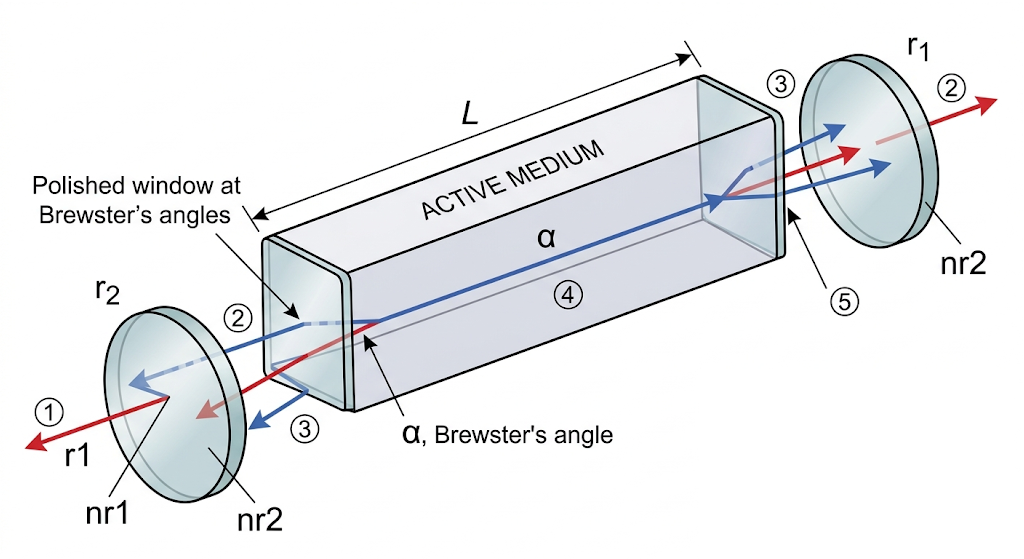
\includegraphics[width=0.88\textwidth]{cavity_scheme.png}
  \caption{Schematic of a gas laser with Brewster windows, central active medium,
    high‑reflectivity mirror (left) and semitransparent output mirror (right).}
  \label{fig:cavity_scheme}
\end{figure}

\subsection{Operating principles — Quantum mechanics of the process}

Electrons in atoms are found in discrete energy levels defined by quantum numbers. In their
ground state, electrons neither absorb nor emit energy. The relation between the energy of
a photon and the frequency of the emitted radiation is given by the Planck-Einstein relation:
%
\begin{equation}
  \Delta E = h\,\nu
  \label{eq:planck}
\end{equation}
%
where $\Delta E$ is the photon energy, $h$ is Planck's constant
($h = 6.626 \times 10^{-34}$\,J$\cdot$s) and $\nu$ is the radiation frequency.

Figure~\ref{fig:energy_levels} illustrates the possible energy transitions between discrete
quantum levels.

\begin{figure}[H]
  \centering
  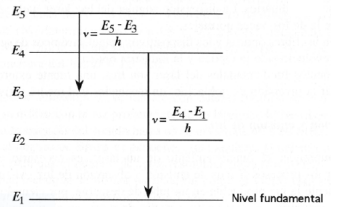
\includegraphics[width=0.58\textwidth]{energy_levels.png}
  \caption{Energy level diagram. Arrows represent electronic transitions with photon
    emission at the corresponding frequencies.}
  \label{fig:energy_levels}
\end{figure}

When electrons absorb energy they jump to a higher level; when they decay to a lower level
they emit photons. Normally, in the active medium, most atoms have their electrons in the
ground state, but some excited atoms spontaneously emit photons upon returning to that
state. This process is random and the emitted photons are neither coherent nor maintain
any phase relationship with each other.

When radiation of suitable energy impinges on an electron in an excited state, the atom
is \textit{stimulated} to emit a photon of the same frequency and phase. By adding both
radiations —the incident and the emitted— \textbf{radiation amplification} occurs
(Figure~\ref{fig:emission_types}).

\begin{figure}[H]
  \centering
  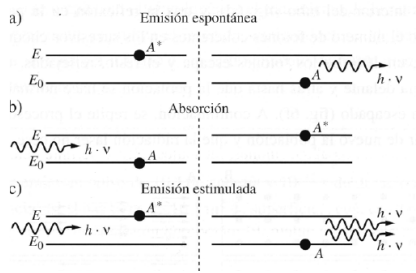
\includegraphics[width=0.72\textwidth]{emission_types.png}
  \caption{The three radiative processes: (a) spontaneous emission, (b) absorption and
    (c) stimulated emission. The latter is the one that sustains laser operation.}
  \label{fig:emission_types}
\end{figure}

Under normal conditions, stimulated emission is a very small effect because few atoms are
in an excited state. For a laser to work, the active medium must have at least three energy
levels and the pumping system must achieve \textbf{population inversion}: bring most atoms
to the excited state, making stimulated emission highly probable
(Figure~\ref{fig:population_inversion}).

\begin{figure}[H]
  \centering
  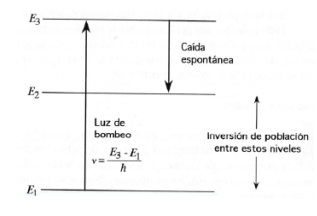
\includegraphics[width=0.52\textwidth]{population_inversion.png}
  \caption{Population inversion in a three‑level system. Pump light promotes electrons
    from $E_1$ to $E_3$; fast spontaneous decay to $E_2$ creates the inversion between
    $E_2$ and $E_1$ needed for stimulated emission.}
  \label{fig:population_inversion}
\end{figure}

The resonant cavity makes the light beams bounce back and forth inside it, generating
phase‑synchronised stimulated emission in pulses tuned to the cavity length $L$
(Figure~\ref{fig:cavity_resonant}).

\begin{figure}[H]
  \centering
  \includegraphics[width=0.88\textwidth]{resonant_cavity.png}
  \caption{Fabry-Pérot resonant cavity. The beam travels round trips
    ($1 \to 2 \to 3 \to 4 \to 5$) being amplified on each pass through the active medium.
    $R_1$: high‑reflectivity rear mirror; $R_2$: semitransparent output coupler.}
  \label{fig:cavity_resonant}
\end{figure}

% ══════════════════════════════════════════════════════════════════════════════
\section{Cavity Threshold Condition}

The \textbf{threshold condition} is the critical point at which the light gain inside the
cavity exactly equals the losses, allowing the laser to begin sustained oscillation. To
establish it, the following variables are defined:

\begin{itemize}[leftmargin=2em]
  \item $\alpha$ \,[cm$^{-1}$]: gain per unit length in the active medium.
  \item $L$ \,[cm]: length of the active material.
  \item $R_1,\, R_2$ \,(dimensionless, $0 < R_i \leq 1$): reflectivities of the two mirrors.
  \item $\phi$ \,[photons/cm$^3$]: photon density in the cavity.
\end{itemize}

Consider a beam travelling parallel to the optical axis. On completing one \emph{round trip}
inside the cavity, the beam experiences:

\begin{enumerate}[leftmargin=2em]
  \item \textbf{Gain:} by traversing the active medium twice (total distance $2L$), the
        photon density is multiplied by the amplification factor $e^{2\alpha L}$.
  \item \textbf{Reflection losses:} by reflecting off both mirrors, the density is reduced
        by the factors $R_1$ and $R_2$.
\end{enumerate}

At threshold, the photon density at the beginning of the cycle $\phi_i$ must equal the
density at the end $\phi_f$:
%
\begin{equation}
  \phi_i \cdot e^{2\alpha L} \cdot R_1 \cdot R_2 = \phi_f
  \label{eq:threshold_full}
\end{equation}
%
Since $\phi_i = \phi_f$ in the steady‑state regime at threshold, this simplifies to:
%
\begin{equation}
  e^{2\alpha L} \cdot R_1 \cdot R_2 = 1
  \quad\Longrightarrow\quad
  e^{-2\alpha L} = R_1 \cdot R_2
  \label{eq:threshold}
\end{equation}

This is the \textbf{exact threshold equation}: a transcendental equation that relates the
gain to the mirror reflectivities.

% ══════════════════════════════════════════════════════════════════════════════
\section{Mathematical Development Using Numerical Series}

\subsection{Taylor series expansion}

At threshold, the gain $\alpha$ is a small quantity, so the product $2\alpha L \ll 1$.
This allows us to approximate the exponential function in equation~\eqref{eq:threshold}
using its Taylor series (Maclaurin series) around the origin. The general exponential
series is:
%
\begin{equation}
  e^{x} = \sum_{n=0}^{\infty} \frac{x^n}{n!}
         = 1 + x + \frac{x^2}{2!} + \frac{x^3}{3!} + \frac{x^4}{4!} + \cdots
\end{equation}
%
Substituting $x = -2\alpha L$ into the threshold equation~\eqref{eq:threshold}:
%
\begin{equation}
  e^{-2\alpha L}
  = \sum_{n=0}^{\infty} \frac{(-2\alpha L)^n}{n!}
  = 1 + (-2\alpha L) + \frac{(-2\alpha L)^2}{2!} + \frac{(-2\alpha L)^3}{3!} + \cdots
  = R_1 R_2
  \label{eq:full_series}
\end{equation}

The series converges for all values of $\alpha L$, and in particular converges absolutely
for $2\alpha L < 1$, a condition that holds in high‑reflectivity industrial lasers.

\subsection{Truncation of the series — physical justification}

Since $\alpha$ is small at threshold, the higher‑order terms are much smaller than the
first ones. Truncating series~\eqref{eq:full_series} after the linear term:
%
\begin{equation}
  \boxed{e^{-2\alpha L} \approx 1 - 2\alpha L}
  \label{eq:linear_approx}
\end{equation}

This approximation has a precise physical interpretation. Each pass through the cavity
provides a small incremental gain; the higher‑order terms of the series correspond to
second‑, third‑ and higher‑order contributions of those accumulated corrections, which
become negligible when $2\alpha L \ll 1$.
Mathematically, the truncation corresponds to the first‑order approximation
$e^{-x} \approx 1 - x$ for $|x| \ll 1$, rigorously justified by the convergence
criterion of the Taylor series.

% ══════════════════════════════════════════════════════════════════════════════
\section{Calculation of the Characteristic Gain}

Substituting the approximation~\eqref{eq:linear_approx} into the threshold condition:
%
\begin{equation}
  1 - 2\alpha_c L = R_1 R_2
\end{equation}

Solving for the \textbf{characteristic gain of the oscillator} $\alpha_c$:
%
\begin{equation}
  \boxed{\alpha_c = \frac{1 - R_1 R_2}{2L}}
  \label{eq:gain}
\end{equation}

This result is the central expression of this work. It is a simple and powerful analytic
formula that directly yields the minimum threshold gain required for the laser to oscillate,
given only the geometric and optical parameters of the cavity.

% ══════════════════════════════════════════════════════════════════════════════
\section{Truncation Error Analysis}

The linear approximation~\eqref{eq:linear_approx} introduces a truncation error whose
dominant term is the quadratic term of the series:
%
\begin{equation}
  \varepsilon_{\rm trunc} \approx \frac{(2\alpha L)^2}{2}
  \label{eq:error}
\end{equation}

The \textit{relative error} with respect to the linear term is of order $\alpha L$:
%
\begin{equation}
  \varepsilon_{\rm rel} \approx \frac{(2\alpha L)^2/2}{2\alpha L} = \alpha L
\end{equation}

\subsection{High reflectivity case — typical industrial lasers}

For a cutting laser with $R_1 = 0.99$, $R_2 = 0.95$ and $L = 10$\,cm:

\begin{align}
  R_1 R_2 &= 0.9405 \\[4pt]
  \alpha_c &= \frac{1 - 0.9405}{2 \times 10} = \frac{0.0595}{20}
            = 2.975 \times 10^{-3}\;\text{cm}^{-1} \\[4pt]
  \varepsilon_{\rm trunc} &= \frac{(2 \times 2.975\times10^{-3} \times 10)^2}{2}
                           = \frac{(0.0595)^2}{2} \approx 1.77 \times 10^{-3}
\end{align}

The quadratic error is three orders of magnitude smaller than the linear term ($0.0595$).
The approximation is excellent.

\subsection{Low reflectivity or very long cavity case}

If $R_1 R_2 = 0.5$ or $L$ is very large, $\alpha$ grows and $2\alpha L$ ceases to be small.
In this regime the linear approximation progressively loses validity.
Table~\ref{tab:error} illustrates the behaviour of the error as a function of the product
$2\alpha L$:

\begin{table}[H]
  \centering
  \caption{Error of the linear approximation as a function of $x = 2\alpha L$.}
  \label{tab:error}
  \begin{tabular}{cccc}
    \toprule
    $x = 2\alpha L$ & $e^{-x}$ (exact) & $1 - x$ (approx.) & Relative error \\
    \midrule
    0.05 & 0.9512 & 0.9500 & 0.13\% \\
    0.10 & 0.9048 & 0.9000 & 0.53\% \\
    0.20 & 0.8187 & 0.8000 & 2.28\% \\
    0.50 & 0.6065 & 0.5000 & 17.6\% \\
    1.00 & 0.3679 & 0.0000 & 100\%    \\
    \bottomrule
  \end{tabular}
\end{table}

For values $x > 0.2$ it is advisable to include at least the quadratic term:
%
\begin{equation}
  e^{-2\alpha L} \approx 1 - 2\alpha L + \frac{(2\alpha L)^2}{2}
  \quad \Longrightarrow \quad
  \frac{(2\alpha_c L)^2}{2} - 2\alpha_c L + (1 - R_1 R_2) = 0
\end{equation}
%
which is a quadratic equation in $\alpha_c$ with an exact analytic solution, or alternatively
solve the transcendental equation~\eqref{eq:threshold} numerically.

% ══════════════════════════════════════════════════════════════════════════════
\section{Discussion}

Expression~\eqref{eq:gain} is the central result of this work. Its derivation directly
links \textbf{advanced calculus} —the theory of Taylor series— with a concrete design
parameter in laser device engineering.

From an industrial design perspective:

\begin{itemize}[leftmargin=2em]
  \item The formula allows a quick estimate of how much gain the active medium must provide
        for the laser to exceed threshold, without having to solve transcendental equations.
  \item The values of $R_1$ and $R_2$ are controllable design parameters (quality of mirror
        coatings), while $L$ is a geometrical parameter of the cavity. The required gain
        $\alpha_c$ guides the choice of the active medium (doping density, amplification length).
  \item In SLM/DMLS processes, where high power density is required, short cavities with
        highly reflective mirrors are preferred, keeping $2\alpha L$ small and validating
        the linear approximation.
\end{itemize}

The convergence of the series and the validity of the linear approximation are justified
by typical high‑reflectivity operating conditions ($R_1 R_2 \gtrsim 0.9$, $x = 2\alpha L \lesssim 0.1$), where the error is below $0.5\%$.

% ══════════════════════════════════════════════════════════════════════════════
\section{Conclusion}

In this work, we have demonstrated the direct application of numerical series
—specifically the Taylor series— to a fundamental problem in laser engineering:
the calculation of resonant cavity gain.

Starting from the physical threshold condition for photon density, we arrived at the
transcendental equation $e^{-2\alpha L} = R_1 R_2$. By expanding this exponential in a
Maclaurin series and truncating to the linear term, we mathematically justified the
approximation $e^{-2\alpha L} \approx 1 - 2\alpha L$, and obtained the analytical
expression for the characteristic gain:
%
\begin{equation*}
  \alpha_c = \frac{1 - R_1 R_2}{2L}
\end{equation*}

The truncation error analysis confirms that the approximation is excellent
(error $< 0.5\%$) for the typical operating conditions of industrial high‑power lasers,
where reflectivities are very high ($R_1 \approx 100\%$, $R_2 \approx 95\%$).

We conclude that advanced calculus, through the use of numerical series, provides essential
tools to model and simplify complex problems in laser device physics. This modelling is
fundamental to determine the minimum energy required to activate an industrial high‑power
laser, thus optimising cutting‑edge metallurgical processes such as selective laser
sintering and high‑precision laser machining.

% ══════════════════════════════════════════════════════════════════════════════
\section*{References}

\begin{enumerate}[leftmargin=2em, label={[\arabic*]}]
  \item Saleh, B.E.A. \& Teich, M.C. (2007). \textit{Fundamentals of Photonics} (2nd ed.).
        Wiley-Interscience. Chap. 15.
  \item Svelto, O. (2010). \textit{Principles of Lasers} (5th ed.). Springer.
  \item Hecht, J. (2018). \textit{The Laser Guidebook} (2nd ed.). McGraw-Hill.
  \item Apostol, T.M. (1967). \textit{Calculus}, Vol. I. Blaisdell. Chap. 11 (Taylor series).
\end{enumerate}

\end{document}